\documentclass{ltxdoc}
\usepackage[linespread=1.5]{ctex}
\usepackage{review}
\usepackage{tcolorbox}
\usepackage{multicol}
\usepackage{geometry}
\geometry{
  left=4cm,
  right=3cm,
  top=2.5cm,
  bottom=2.5cm
}
\usepackage{enumitem}
\newlist{options}{description}{1}
\setlist[options]{font=\normalfont}
\usepackage{tikz}
\usetikzlibrary{positioning, fit}
\usepackage{fancyvrb-ex}
\usepackage{booktabs}
\usepackage{array}
\usepackage[numbered]{hypdoc}
\hypersetup{
  bookmarksopen,
  bookmarksopenlevel=3,
}

\makeatletter
\renewcommand*\title[2][]{\gdef\@title{#2}}
\renewcommand*\author[2][]{\gdef\@author{#2}}
\@ifundefined{call}{\def\call#1{#1}}{}
\def\SpecialCallIndex#1{\@bsphack
   {\let\special@index\index\SpecialIndex@{#1}{\encapchar call}}%
   \@esphack}
\let\HDorg@SpecialCallIndex\SpecialCallIndex
\renewcommand*\SpecialCallIndex[1]{%
  \@bsphack
  \begingroup
    \HD@target
    \let\index\HDorg@index
    \let\HDorg@encapchar\encapchar
    \edef\encapchar call{%
       \HDorg@encapchar hdclindex{\the\c@HD@hypercount}{call}%
    }%
    \HDorg@SpecialCallIndex{#1}%
  \endgroup
  \@esphack
}
\DeclareRobustCommand\oiarg[1]{%
     {\normalfont\ttfamily[}%
     \ifmmode \expandafter \nfss@text \fi
     {%
      \meta@font@select
      \edef\meta@hyphen@restore
        {\hyphenchar\the\font\the\hyphenchar\font}%
      \hyphenchar\font\m@ne
      \language\l@nohyphenation
      #1\/%
      \meta@hyphen@restore
     }{\normalfont\ttfamily]}%
}
\makeatother
\providecommand\alert[1]{\textcolor{red}{#1}}

\tikzset{
  prop/.style={
    minimum width=1cm,
    minimum height=3mm,
    draw, fill=purple!60,
  },
  fit outer/.style={
    inner xsep=5mm,
    inner ysep=3mm,
    fit={#1}, draw, fill=yellow!20,
  },
  fit inner/.style={
    inner xsep=2mm,
    inner ysep=1.5mm,
    fit={#1}, draw, fill=cyan!50,
  },
}
\pgfdeclarelayer{back}
\pgfdeclarelayer{fore}
\pgfsetlayers{back, main, fore}

\rvsetclass{math}
\rvsetupall{
  global-group=star,
  group={test},
  prop={date, content, count},
}
\rvnewreviewpoint{default}{2, 5}
\def\mydate{2020-10-01}

\DeclarervGroupEnvironment { math } { m +b }
  {
    \rvifreviewT{default}{\mydate}{#1}
      {
        \rvcstep*{test}
        \rvesave*{test}{count}{\rvcAlph*{test}}
        \rvsave*{test}{date}{#1}
        \rvaddtogroup{test}
      }
    \NewDocumentCommand { \mysave } { s m }
      {
        \IfBooleanT { ##1 }
          {
            \rvesave*{star}{count}{\rvcAlph*{test}}
            \rvsave*{star}{content}{##2}
          }
        \rvcstep{test}
        \rvesave{test}{count}{\rvcAlph{test}}
        \rvsave{test}{content}{##2}
      }
    #2
  } { }

\rvsetshowstyle*{math}{star}{content}
  {\begin{tcolorbox}\begin{multicols}{2}}
  {\end{multicols}\end{tcolorbox}}
  {
    saved counter:~\rvuse{count}\par
    rvitem:~\rvcRoman{rvitem}\par
    content:~\rvuse{content}\par
    \vspace{1em}
  }

\rvsetshowstyle{math}{test}{content}
  {\begin{tcolorbox}\begin{multicols}{2}}
  {\end{multicols}\end{tcolorbox}}
  {
    \begin{tcolorbox}[colback=yellow!20, title={\rvuse[test]{date}}]
  }
  {\end{tcolorbox}}
  {
    saved counter:~\rvuse{count}\par
    rvitem:~\rvcRoman{rvitem}\par
    content:~\rvuse{content}\par
    \vspace{1em}
  }

\IndexPrologue{%
  \section*{索引}
  \markboth{索引}
  斜体的数字表示对应项说明所在的页码;下划线的数字表示定义所在的代码行号;而
  直立体的数字表示对应项使用时所在的行号。
}

\AtBeginDocument{%
  \DeleteShortVerb{\|}%
  \MakeShortVerb{\"}%
}
\AtEndDocument{\PrintIndex}
\CodelineIndex\EnableCrossrefs%

\title[review宏包]{\texttt{review}宏包\footnote{\url{https:%
//github.com/ZhiyuanLck/review}}(v1.0)}
\author[李昌锴 <lichangkai225@qq.com>]{李昌锴\\[.5em]\path{lichangkai225@qq.com}}
\date{2020/10/05}

\begin{document}

\maketitle

\section{简介}
编写 "review"宏包的初衷是为了整合之前写的两个复习错题的模板,但是抛弃了对样式
的定制(交给使用者自己定制)以及拓展了更为广泛的用途。收录错题并按照复习日期或
者其他条件展示错题本质上是对数据的存储和使用,"review"宏包将这些存取逻辑抽象了
出来并提供了接口供用户使用。

如果仅仅是从数据的读写角度,用户可能有更好的选择比如 "datatool"宏包提供了数据
库相关的更为一般的方法。但是从使用 \LaTeX 的角度来看,存储数据最终都会按照一
定样式展示出来。"review"宏包定义了数据库相关的概念("class"对应数据库,"group"
对应表和 "property"对应属性),提供了更为简化的命令可以方便快捷地定义数据结构,
对数据进行存取操作,以及以 "group"为单位定义数据展示样式。此外通过区分
"local group"与 "global group"实现了类似数据库中通过 "groupby" 查询数据的功能。

\section{使用}

\subsection{相关概念}

\subsubsection*{"class"}
"class"相当于是一个数据库,一个文档内可以有多个 "class",每一个 "class"都可以
定义一个与之相对应的 "GroupEnvironment",在环境定义中完成对数据的存储。

\subsubsection*{"group"}
每个 "class"中有若干个数据表,称之为 "group"。 "group"有 "global"和 "local"的
区别。存储数据的时候,如果选择将数据存储存储到 "global group"中,数据会被直接
添加到 "global group"对应的列表中;如果选择将数据存储到 "local group"中,数据
会先被添加到局部于 "GroupEnvironment"的 "subgroup"中,环境结束的时候,
"subgroup"的序号会被添加到 "local group"对应的列表中,这个过程可以理解为所有
在 "GroupEnvironment"中存储到同一个 "local group"中相同类型的数据先被打包成一
个 "subgroup",然后再将这个 "subgroup"添加到 "local group"对应的列表中。
\begin{center}
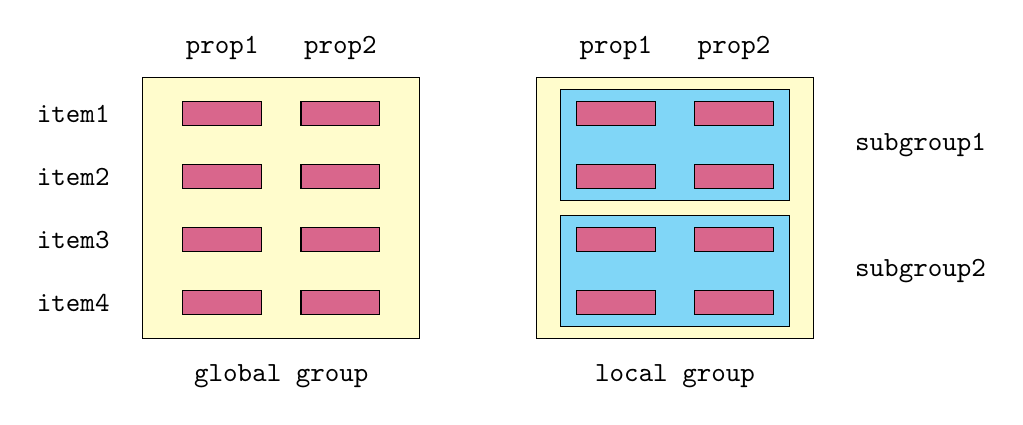
\begin{tikzpicture}[font=\ttfamily]
\foreach \i in { 1,...,2 } {
  \foreach \j in { 1,...,4 } {
    \begin{pgfonlayer}{fore}
      \node[prop] (a-\j-\i) at (\i*1.5, -\j*0.8) {};
    \end{pgfonlayer}
  }
}
\foreach \i in { 1,...,2 } {
  \foreach \j in { 1,...,4 } {
    \begin{pgfonlayer}{fore}
      \node[prop] (b-\j-\i) at ([xshift=5cm]\i*1.5, -\j*0.8) {};
    \end{pgfonlayer}
  }
}
\begin{pgfonlayer}{back}
  \node[fit outer={(a-1-1)(a-4-2)}] (c) {};
  \node[fit outer={(b-1-1)(b-4-2)}] (d) {};
\end{pgfonlayer}
\node[fit inner={(b-1-1)(b-2-2)}] (e) {};
\node[fit inner={(b-3-1)(b-4-2)}] (f) {};

\node[above=4mm of a-1-1] {prop1};
\node[above=4mm of a-1-2] {prop2};
\node[above=4mm of b-1-1] {prop1};
\node[above=4mm of b-1-2] {prop2};
\foreach \i in { 1,...,4 }
  \node[left=8mm of a-\i-1] {item\i};
\node[below=2mm of c] {global group};
\node[below=2mm of d] {local group};
\node[right=7mm of e] {subgroup1};
\node[right=7mm of f] {subgroup2};
\end{tikzpicture}
\end{center}

\subsubsection*{"prop"}
每张数据表中都有若干个属性即 "prop",数据或者说宏都会存储到 "group"中的 "prop"
里。

\subsection{定义数据库结构}
\DescribeMacro{\rvsetclass}
首先使用 "\rvsetclass"\marg{class list}设置 "class"的名字:
\begin{Verbatim}
\rvsetclass{math, en, politics, memo}
\end{Verbatim}
\DescribeMacro{\rvsetupsub}
接着就可以使用 "\rvsetupsub"\marg{class list}\marg{options}将选项应用到
\meta{class list} 中的每个 \meta{class}。
\DescribeMacro{\rvsetupall}
宏包还提供了 "\rvsetupall"\marg{options}将选项应用于已定义的每个 \meta{class}。
可用的选项有:
\begin{options}[labelindent=2\ccwd]
  \item["global-group = "\marg{global group list}]
  \item["local-group = "\marg{local group list}]
  \item["group = "\marg{group list}] 同时设置 "global group" 和 "local group"
  \item["global-counter = "\marg{global counter list}]
  \item["local-counter = "\marg{local counter list}]
  \item["counter = "\marg{counter list}] 同时设置 "global counter" 和 "local counter"
\end{options}

\subsection[定义GroupEnvironment]{定义 "GroupEnvironment"}
宏包提供了几乎与 "xparse"宏包一致的定义环境的命令\\
\SpecialUsageIndex{\NewrvGroupEnvironment}
"\NewrvGroupEnvironment" \marg{key-val list} \marg{arg spec}\\
\mbox{}\quad\marg{start code} \marg{end code}\\
唯一不同的是第一个必选参数,其中 \meta{key-val} 的格式是 \meta{class name
\oiarg{= env name}} , \meta{class name} 的形式会被自动转化成 \meta{class name
= rv\meta{class name}}。即将 "GroupEnvironment"与 "class"关联起来,这样在
"GroupEnvironment"中对 "group","prop","counter"的操作都被关联到对应的
"class"上。该命令为不同 "class"的 "GroupEnvironment"设置作用一致的代码。环境
定义的详细用法请参照 "xparse"宏包的使用文档。
\begin{Verbatim}
\NewrvGroupEnvironment { math, en=myen } { +b }
  { #1 } { }
\begin{document}
\begin{rvmath}
  ...
\end{rvmath}

\begin{myen}
  ...
\end{myen}
\end{document}
\end{Verbatim}

与 "xparse"宏包一样,其他变种命令也是可用的,具体的区别请参考 "xparse"宏包的使
用文档。\\
"\RenewrvGroupEnvironment"\SpecialUsageIndex{\RenewrvGroupEnvironment}\\
"\DeclarervGroupEnvironment"\SpecialUsageIndex{\DeclarervGroupEnvironment}\\
"\ProvidervGroupEnvironment"\SpecialUsageIndex{\ProvidervGroupEnvironment}

\subsection{存储数据和使用数据}
\DescribeMacro{\rvsave}
使用 "\rvsave" \marg {global group} \marg{prop} \marg{content} 将数据存储到
\meta{local group} 的属性 \meta{prop} 中,
\DescribeMacro{\rvsave*}
或者使用 "\rvsave*" \marg{local group} \marg{prop} \marg{content} 将数据存储到
\meta{local group} 的属性 \meta{prop} 中。
\DescribeMacro{\rvesave}
同时宏包还提供了变异的命令 "\rvesave"和 "\rvesave*",与 "\rvsave"和 "\rvsave*"
\DescribeMacro{\rvesave*}
作用一致,唯一不同的是 \meta{content} 先被完全展开再存储到对应的 \meta{prop}
中。这些命令只在 "GroupEnvironment"中可用。

存储到 "local group"中的数据先被打包成一个 "subgroup"然后添加到对应的列表中,
\DescribeMacro{\rvaddtogroup}
宏包提供了命令 "\rvaddtogroup" \marg{local group list} 来控制这个过程,即把当
前的 "subgroup"添加到 \meta{local list} 对应的列表中,如果不使用这个命令,最
终展示 "local group"的时候会忽略这个 "subgroup",多次添加会导致同一个
"subgroup"被打印多次,也可能导致本应同步的 "global group"和 "local group"最终
变得不同步(见 \ref{sec:sync} 节)。

\DescribeMacro{\rvuse}
使用 "\rvuse" \oarg{global group} \marg{prop} 来获取对应 \meta{prop} 的值,对
应的 "class" ,"group" 以及列表的索引都是根据当前环境自动获取的。
在 "\rvsetshowstyle" 中 "group"被自动设置为对应的 "global group",
在 "\rvsetshowstyle*" 中 "group"被自动设置为对应的 "local group"。
可选参数 \meta{global group} 用于在展示 "local group" 的时候获取与之同步(见
\ref{sec:sync} 节)的 "global group"中 \meta{prop} 的值,因此在
"\rvsetshowstyle" \SpecialCallIndex{\rvsetshowstyle}中这个可选参数会被忽略。
使用数据的命令只在 "\rvsetshowstyle"或者
"\rvsetshowstyle*"\SpecialCallIndex{\rvsetshowstyle*}(见 \ref{sec:show} 节)
中可用。

\subsection{定义展示样式}\label{sec:show}
\subsubsection*{定义 "global group"的展示样式}
\noindent
\DescribeMacro{\rvsetshowstyle}
"\rvsetshowstyle" \marg{class list} \marg{global group list}
\marg{anchor prop}\\
\mbox{}\quad\marg{before group code} \marg{after group code}\\
\mbox{}\quad\marg{item code}

该命令假设 \meta{class list} 中的所有 \meta{class} 都有共同的
\meta{global group} 且为这些 \meta{global group} 设置相同的样式。最终显示的
\meta{item} 的数量与 \meta{anchor prop} 对应的列表的长度相同。

\subsubsection*{定义 "local group"的展示样式}
\noindent
\DescribeMacro{\rvsetshowstyle*}
"\rvsetshowstyle*" \marg{class list} \marg{local group list}
\marg{anchor prop}\\
\mbox{}\quad\marg{before group code} \marg{after group code}\\
\mbox{}\quad\marg{before subgroup code} \marg{after subgroup code}\\
\mbox{}\quad\marg{item code}

该命令假设 \meta{class list} 中的所有 \meta{class} 都有共同的
\meta{local group} 且为这些 \meta{local group} 设置相同的样式。 "subgroup"中最终显示的
\meta{item} 的数量与同一个 "subgroup"中 \meta{anchor prop} 对应的列表的长度相
同。与 "global group"不同的是, "local group"中的数据以样式相同的 "subgroup"的
形式进行展示。

\subsubsection*{展示 "group"}
\DescribeMacro{\rvshow}
使用 "\rvshow" \marg{class} \marg{local group} 或者 "\rvshow*" \marg{class}
\marg{global group} 将 "group"以定制好的样式打印出来。
\DescribeMacro{\rvshow*}


\subsection{组同步} \label{sec:sync}
可以通过让 "global group"与 "local group"同步从而存储与 "subgroup"相关的信息,
同步是指当且仅当在使用
"\rvaddtogroup"\SpecialCallIndex{\rvaddtogroup} 的时候才进行一次对
"global group"的数据存储操作(相同 "prop"只进行一次存储操作)。

\begin{center}
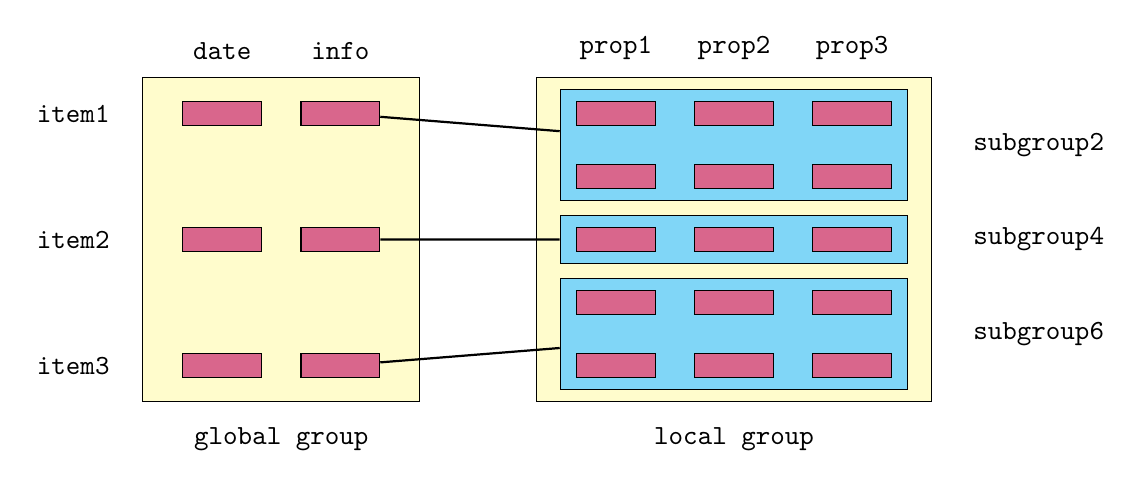
\begin{tikzpicture}[font=\ttfamily]
\foreach \i in { 1,...,2 } {
  \foreach \j in { 1,...,3 } {
    \begin{pgfonlayer}{fore}
      \node[prop] (a-\j-\i) at (\i*1.5, -\j*1.6) {};
    \end{pgfonlayer}
  }
}
\foreach \i in { 1,...,3 } {
  \foreach \j in { 1,...,5 } {
    \begin{pgfonlayer}{fore}
      \node[prop] (b-\j-\i) at ([shift={(5, -0.8)}]\i*1.5, -\j*0.8) {};
    \end{pgfonlayer}
  }
}
\begin{pgfonlayer}{back}
  \node[fit outer={(a-1-1)(a-3-2)}] (c) {};
  \node[fit outer={(b-1-1)(b-5-3)}] (d) {};
\end{pgfonlayer}
\node[fit inner={(b-1-1)(b-2-3)}] (e) {};
\node[fit inner={(b-3-1)(b-3-3)}] (f) {};
\node[fit inner={(b-4-1)(b-5-3)}] (g) {};

\node[above=4mm of a-1-1] {date};
\node[above=4mm of a-1-2] {info};
\node[above=4mm of b-1-1] {prop1};
\node[above=4mm of b-1-2] {prop2};
\node[above=4mm of b-1-3] {prop3};
\foreach \i in { 1,...,3 }
  \node[left=8mm of a-\i-1] {item\i};
\node[below=2mm of c] {global group};
\node[below=2mm of d] {local group};
\node[right=7mm of e] {subgroup2};
\node[right=7mm of f] {subgroup4};
\node[right=7mm of g] {subgroup6};
\begin{scope}[thick]
  \draw (a-1-2) -- (e);
  \draw (a-2-2) -- (f);
  \draw (a-3-2) -- (g);
\end{scope}
\end{tikzpicture}
\end{center}

下面给出了和上图对应的组同步的示例:
\begin{Verbatim}
\rvsetclass{math}
\rvsetupall{
  group=sync,
  prop={date, info, prop1, prop2, prop3}
}
% #1 state number #2 date #3 info
\NewrvGroupEnvironment { math } { m m m +b }
  {
    \ifodd#1\else%
      \rvaddtogroup{sync}%
      \rvsave*{sync}{date}{#2}%
      \rvsave*{sync}{info}{#3}%
    \fi%
    \newcommand\savetosync[3]{%
      \rvsave{sync}{prop1}{##1}%
      \rvsave{sync}{prop2}{##2}%
      \rvsave{sync}{prop3}{##3}%
    }%
    #4
  } { }
\begin{document}
\begin{rvmath}{2}{2020-09-08}{no}
  \savetosync{val1-1}{val1-2}{val1-3}
  \savetosync{val2-1}{val2-2}{val2-3}
\end{rvmath}
\begin{rvmath}{4}{2020-09-03}{no}
  \savetosync{val1-1}{val1-2}{val1-3}
\end{rvmath}
\end{document}
\end{Verbatim}

\subsection{计数器}

\subsubsection{简介}
在 "\rvsetupsub"\SpecialCallIndex{\rvsetupsub} 和
"\rvsetupall"\SpecialCallIndex{\rvsetupall} 中你可以使用选项
"global-counter", "local-counter"或者 "counter"为不同的 "class"设置计数器。不
同的 "class"可以使用相同名称的计数器,甚至不同作用范围的计数器也可以使用相同
的名称,但实际上这些计数器都是互不相同的。全局计数器作用于全局,在定义
"GroupEnvironment"的时候初始化为$0$;局部计数器局部于 "GroupEnvironment",在使
用 "GroupEnvironment"之前初始化为$0$。

宏包为每个 "global group"设置了与其名称相同的全局计数器,为每个 "local group"
设置了与其名称相同的局部计数器和全局计数器(用于同步)。

\subsubsection{保留计数器}
计数器名称rvenv,rvitem,rvgroup是保留给宏包的名称,如果出现在计数器相关的选项中会
提示错误。这三个计数器是\alert{只读}的。
\begin{itemize}[font=\sffamily]
  \item[rvenv] 只能在 "GroupEnvironment"中使用,计数 "GroupEnvironment"的使用
    次数。
  \item[rvitem] 只能在 "\rvsetshowstyle"\SpecialCallIndex{\rvsetshowstyle} 和
    "\rvsetshowstyle*"\SpecialCallIndex{\rvsetshowstyle*} 中使用,计数当前
    "item"的数量。
  \item[rvgroup] 只能在 "\rvsetshowstyle"\SpecialCallIndex{\rvsetshowstyle} 中
    使用,计数当前 "subgroup"的数量。
\end{itemize}

\subsubsection{计数器使用}
计数器相关的命令都以 "rvc"开头,星号版本代表对全局的计数器进行操作,否则代表
对局部的计数器进行操作,表 \ref{tab:counter} 列出了不同的计数方式对应的命令。
此外还可以通过 "\rvcvalue" \marg{local counter}\DescribeMacro{\rvcvalue} 或者
"\rvcvalue*" \marg{global counter} 来获取对应计数器的值,两个命令均可以获取保%
\DescribeMacro{\rvcvalue*}%
留计数器的值,得到的结果相同。这些命令都可以在 "GroupEnvironment"或者
"\rvsetshowstyle"\SpecialCallIndex{\rvsetshowstyle}
和 "\rvsetshowstyle*"\SpecialCallIndex{\rvsetshowstyle*} 中使用,但要注意将计
数器的值作为数据存储的时候要使用 "\rvesave"\SpecialCallIndex{\rvesave} 或者
"\rvesave*"\SpecialCallIndex{\rvesave*}。

\begin{table}[ht]
\centering
\caption{不同计数方式对应的命令}
\label{tab:counter}
\vskip1em
\begin{tabular}{ll>{\rule{1cm}{0pt}}l}
  \toprule
  "\rvarabic" \marg{local counter}\SpecialUsageIndex{\rvarabic} &
  "\rvarabic*" \marg{global counter}\SpecialUsageIndex{\rvarabic*} & 1 2 3 4\\
  "\rvalph" \marg{local counter}\SpecialUsageIndex{\rvalph} &
  "\rvalph*" \marg{global counter}\SpecialUsageIndex{\rvalph*} & a b c d\\
  "\rvAlph" \marg{local counter}\SpecialUsageIndex{\rvAlph} &
  "\rvAlph*" \marg{global counter}\SpecialUsageIndex{\rvAlph*} & A B C D\\
  "\rvroman" \marg{local counter}\SpecialUsageIndex{\rvroman} &
  "\rvroman*" \marg{global counter}\SpecialUsageIndex{\rvroman*} & i ii iii iv\\
  "\rvRoman" \marg{local counter}\SpecialUsageIndex{\rvRoman} &
  "\rvRoman*" \marg{global counter}\SpecialUsageIndex{\rvRoman*} & I II III IV\\
  \bottomrule
\end{tabular}
\end{table}

\DescribeMacro{\rvcstep}
使用 "\rvcstep" \marg{local counter} 或者 "\rvcstep*" \marg{global counter} 使
对应计数器的值增加$1$。注意此命令不可用于保留计数器,且只能在
\DescribeMacro{\rvcstep*}
"GroupEnvironment"中使用。

\DescribeMacro{\rvcset}
使用 "\rvcset" \marg{local counter} \marg{integer expr} 或者 "\rvcset*"
\marg{global counter} \marg{integer expr} 将对应计数器的值设置为整数表达式的%
\DescribeMacro{\rvcset*}
值。注意此命令不可用于保留计数器,且只能在 "GroupEnvironment"中使用。

\subsection{筛选条件}
\subsubsection{通过时间筛选}
\DescribeMacro{\rvnewreviewpoint}
宏包提供了命令 "\rvnewreviewpoint" \marg{review point name} \marg{integer list}
定义新的复习计划(相隔多少天就复习一次)。
\begin{Verbatim}
\rvnewreviewpoint{default}{2, 4, 7, 14, 30, 60}
\end{Verbatim}
同时提供了如下 "if"判断语句来判断 \meta{date-A} 和 \meta{date-B} 的间隔
(\meta{date-A} 在前,\meta{date-B} 在后)是否满足复习计划的设定:\\
\DescribeMacro{\rvifreviewTF}
"\rvifreviewTF" \marg{review point} \marg{date-A} \marg{date-B}
\marg{true code} \marg{false code}\\
\DescribeMacro{\rvifreviewT}
"\rvifreviewT" \marg{review point} \marg{date-A} \marg{date-B}
\marg{true code}\\
\DescribeMacro{\rvifreviewF}
"\rvifreviewF" \marg{review point} \marg{date-A} \marg{date-B}
\marg{false code}

\section{示例}
下面是一个使用示例,定义了 "global group star"用来存放星标的数据,定义了
"local group test"用来按复习日期分组存放数据,以及 "global group test"用来存放
同步的日期。
\begin{Verbatim}
\documentclass{ctexart}
\usepackage{review}
\usepackage{tikz}
\usepackage{multicol}
\usepackage{tcolorbox}

\rvsetclass{math}
\rvsetupall{
  global-group=star,
  group={test},
  prop={date, content, count},
}
\rvnewreviewpoint{default}{2, 5}
\def\mydate{2020-10-01}

\DeclarervGroupEnvironment { math } { m +b }
  {
    \rvifreviewT{default}{\mydate}{#1}
      {
        \rvcstep*{test}
        \rvesave*{test}{count}{\rvcAlph*{test}}
        \rvsave*{test}{date}{#1}
        \rvaddtogroup{test}
      }
    \NewDocumentCommand { \mysave } { s m }
      {
        \IfBooleanT { ##1 }
          {
            \rvesave*{star}{count}{\rvcAlph*{test}}
            \rvsave*{star}{content}{##2}
          }
        \rvcstep{test}
        \rvesave{test}{count}{\rvcAlph{test}}
        \rvsave{test}{content}{##2}
      }
    #2
  } { }

\rvsetshowstyle*{math}{star}{content}
  {\begin{tcolorbox}\begin{multicols}{2}}
  {\end{multicols}\end{tcolorbox}}
  {
    saved counter:~\rvuse{count}\par
    rvitem:~\rvcRoman{rvitem}\par
    content:~\rvuse{content}\par
    \vspace{1em}
  }

\rvsetshowstyle{math}{test}{content}
  {\begin{tcolorbox}\begin{multicols}{2}}
  {\end{multicols}\end{tcolorbox}}
  {
    \begin{tcolorbox}[colback=yellow!20, title={\rvuse[test]{date}}]
  }
  {\end{tcolorbox}}
  {
    saved counter:~\rvuse{count}\par
    rvitem:~\rvcRoman{rvitem}\par
    content:~\rvuse{content}\par
    \vspace{1em}
  }

\begin{document}
\begin{rvmath}{2020-10-03}
  \mysave{test 1}
  \mysave*{test 2}
\end{rvmath}

\begin{rvmath}{2020-10-04}
  \mysave{test 3}
  \mysave*{test 4}
\end{rvmath}

\begin{rvmath}{2020-10-06}
  \mysave{test 5}
  \mysave*{test 6}
\end{rvmath}
\rvshow*{math}{star}
\rvshow{math}{test}
\end{document}

\end{Verbatim}

\begin{rvmath}{2020-10-03}
  \mysave{test 1}
  \mysave*{test 2}
\end{rvmath}

\begin{rvmath}{2020-10-04}
  \mysave{test 3}
  \mysave*{test 4}
\end{rvmath}

\begin{rvmath}{2020-10-06}
  \mysave{test 5}
  \mysave*{test 6}
\end{rvmath}
\rvshow*{math}{star}
\rvshow{math}{test}

\clearpage

\end{document}
